\documentclass[11pt,a4paper]{article}
\usepackage[utf8]{inputenc}\usepackage[T1]{fontenc}
\usepackage[margin=1in]{geometry}
\usepackage{amsmath,amssymb,booktabs,graphicx,enumitem,xcolor,parskip,titlesec}
\usepackage[hidelinks]{hyperref}
\graphicspath{{figures/}}
\definecolor{qnavy}{RGB}{20,40,75}\definecolor{qgrey}{RGB}{90,90,90}\definecolor{qred}{RGB}{150,30,30}
\titleformat{\section}{\large\bfseries\color{qnavy}}{\thesection}{0.6em}{}
\begin{document}\thispagestyle{empty}
\noindent
{\large\bfseries\color{qnavy} Report R17 --- The Genome-Wide Null Was Not a Supervision Artefact}\\[2pt]
{\color{qgrey}R15 concluded that its genome-wide negative came from supervising the wrong target.
Re-running the identical scan on a methylation-supervised representation does not reverse it.
This report corrects R15.}\\[6pt]
{\color{qgrey}\rule{\textwidth}{0.4pt}}

\medskip
\noindent 17 August 2026 \quad\textbullet\quad Quantara \quad\textbullet\quad
{\color{qgrey}Peer-review audit copy}

\section*{Summary}

R15 asked whether H\&E morphology carries methylation information. Its first arm supervised an
attention-MIL on subtype, then asked the resulting embedding about methylation, and found nothing:
genome-wide median $\rho = 0.006$, 110{,}212 of 399{,}579 CpGs above a permutation null, against
220{,}925 for the subtype label by itself. Supervising the same architecture directly on six
aggregate methylation targets recovered partial $\rho$ 0.135--0.244, and R15's audit concluded
that the first negative had been \emph{an artefact of our own supervision choice}.

R15 was explicit that it had not tested this genome-wide --- its limitations state that
``per-CpG prediction under methylation supervision was not attempted''. This report attempts it.

\textbf{The conclusion does not survive.} On the identical scan --- same 760 patients in the same
order, same site-grouped folds, same ridge, same probe filter, only the embedding changing --- the
methylation-supervised representation puts \textbf{83{,}369} CpGs above the null (20.9\%) against
\textbf{90{,}137} for the subtype-supervised one (22.6\%). It is not better. It is slightly worse,
and its median $\rho$ of 0.0073 against 0.0057 is the same flat nothing.

\textbf{Verdict: ARM1\_NEGATIVE\_ROBUST\_TO\_SUPERVISION}, with the secondary verdict
\textbf{GLOBAL\_AXIS\_ONLY}. Both were pre-declared as mechanical rules in the config, hashed at
\texttt{4779152747f14818\ldots} before any arm was computed.

So R15's aggregate-target result stands and its \emph{explanation} of the negative does not. What
the methylation-supervised model learned was the aggregate targets, not the methylome.

\section{Why the comparison is trustworthy before reading it}

The whole claim rests on a reimplementation, so the reimplementation was gated against the
original before the new arm was allowed to count.

\begin{itemize}[leftmargin=1.3em,itemsep=2pt]
\item \textbf{The vectorised Spearman is exact.} R15 looped \texttt{scipy.stats.spearmanr} over
      399{,}579 CpGs; this run rank-transforms and takes Pearson, which is equivalent. Gate G5
      checks it against scipy on 200 real columns: maximum absolute deviation
      $2.1\times10^{-8}$.
\item \textbf{It reproduces R15's per-CpG vectors.} Gate G4 requires $r > 0.999$ against R15's
      saved \texttt{per\_cpg\_rho} arrays. Observed: $r = 1.000000$ for both the subtype-supervised
      embedding and the subtype label.
\item \textbf{It reproduces R15's headline counts to the unit.} On R15's own null threshold
      (0.04605): 110{,}212 and 220{,}925, exactly the published numbers (Figure~C).
\item \textbf{The folds nest.} Rather than re-deriving cross-validation folds, this run takes
      \texttt{fold\_of} as written by the MIL itself, and gate G1 verifies it equals
      \texttt{GroupKFold(5)} grouped by tissue-source site and is identical across both arms. The
      ridge folds are therefore the same folds the representation was trained under, so a
      patient's embedding never comes from a model that saw that patient.
\end{itemize}

Only after all four passed was the new arm computed.

\begin{center}
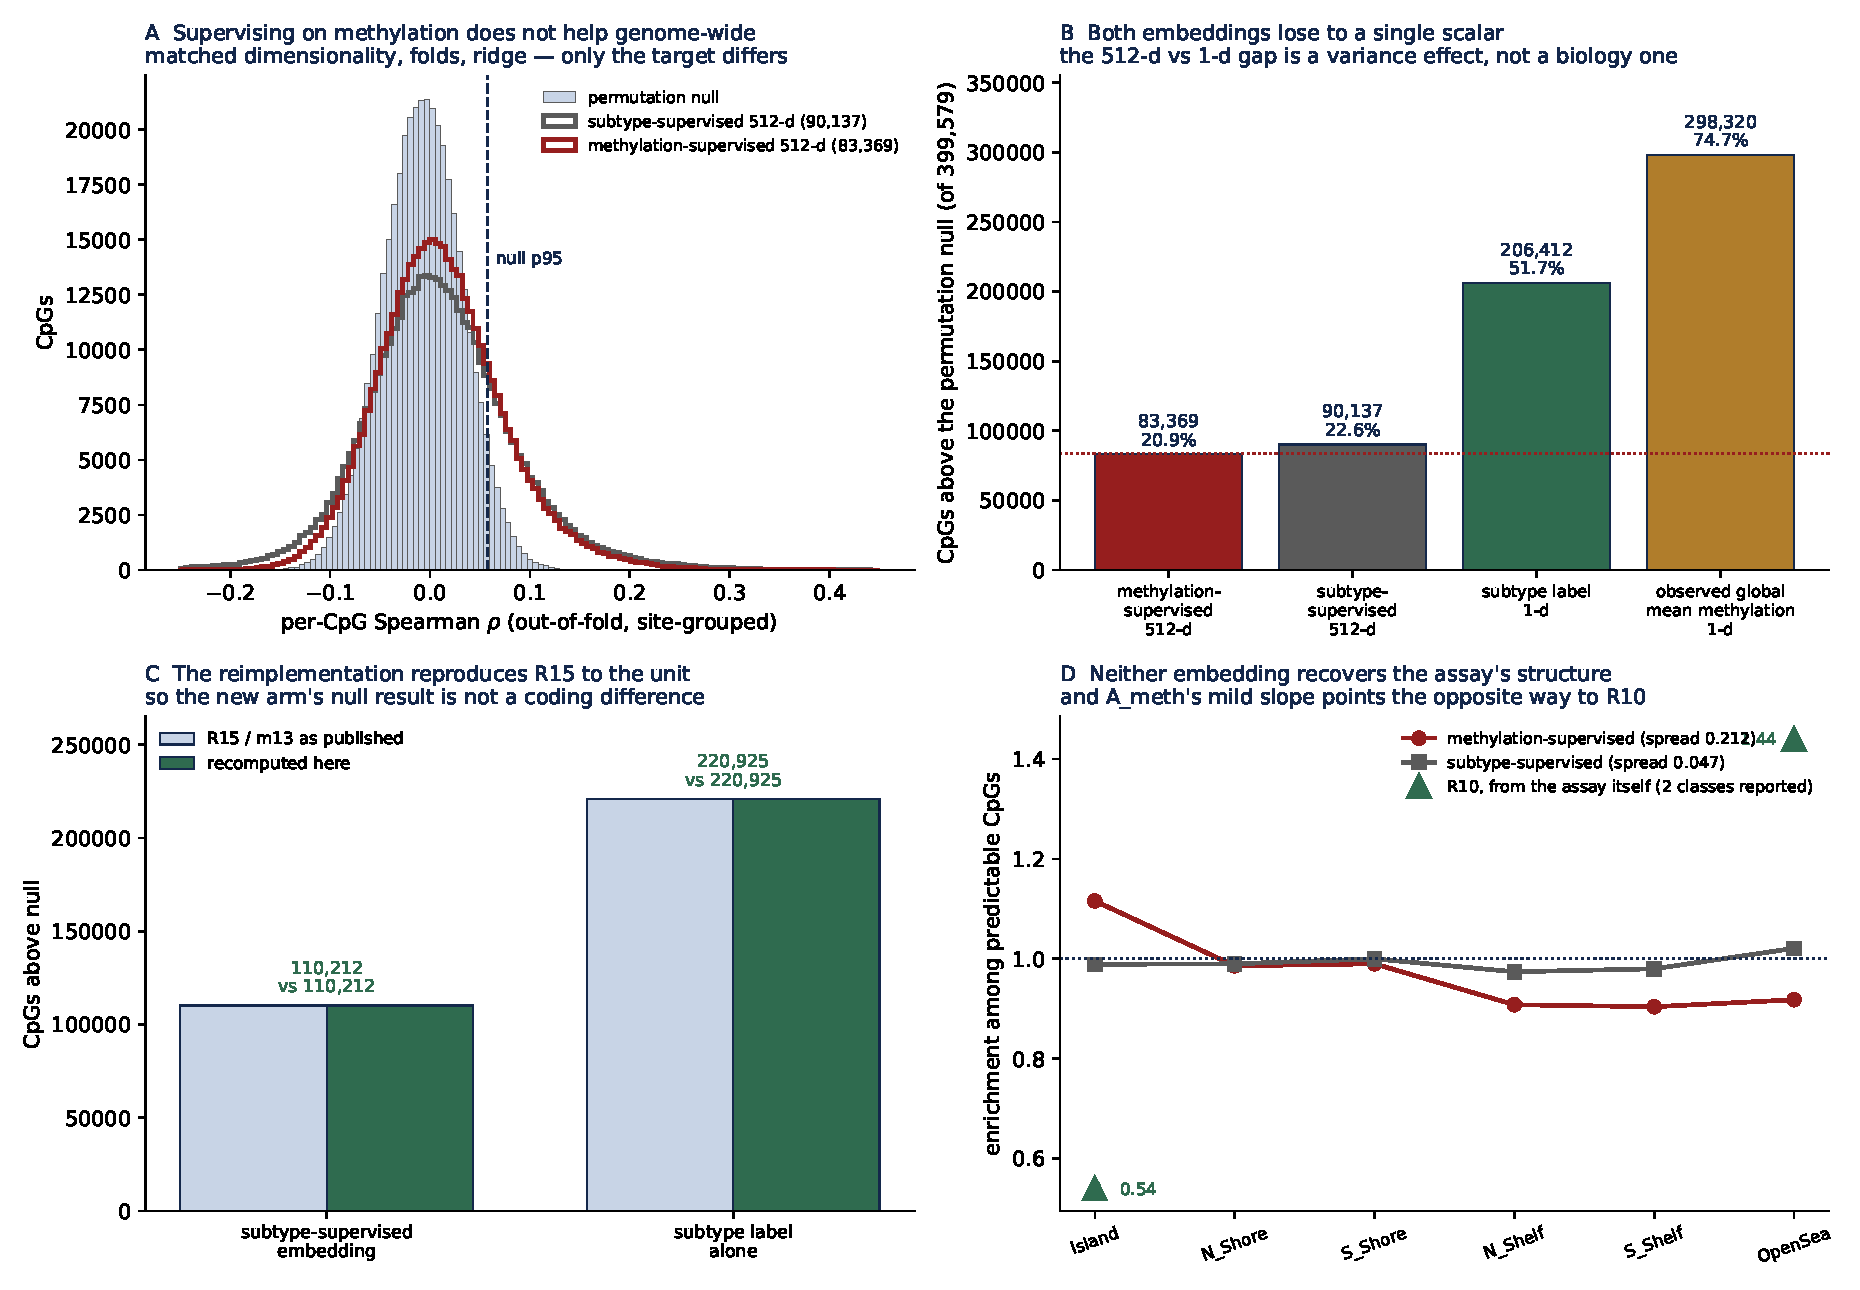
\includegraphics[width=\textwidth]{r17_panels.pdf}
\end{center}
\noindent{\small\color{qgrey}\textbf{A} The decisive comparison: matched dimensionality, folds and
ridge, only the supervision target differing. \textbf{B} All four arms. \textbf{C} The
reimplementation against R15 as published. \textbf{D} Genomic context of the predictable CpGs.}

\section{Results}

\begin{center}
\begin{tabular}{@{}llrrrr@{}}
\toprule
\textbf{Arm} & \textbf{Predictor} & \textbf{dim} & \textbf{above null} & \textbf{\%} &
\textbf{median $\rho$} \\
\midrule
A\_meth & methylation-supervised embedding & 512 & 83{,}369 & 20.9 & 0.0073 \\
A\_sub & subtype-supervised embedding & 512 & 90{,}137 & 22.6 & 0.0057 \\
\midrule
A\_sublabel & LUAD/LUSC label & 1 & 206{,}412 & 51.7 & 0.0631 \\
A\_globalmean & \emph{observed} global mean methylation & 1 & 298{,}320 & 74.7 & 0.2087 \\
\bottomrule
\end{tabular}
\end{center}

\noindent Threshold: 95th percentile of the permutation null, 0.05763; null median $-0.0071$.

\subsection{The two 512-d arms are the finding}

They differ in one respect and agree in outcome. Supervising on methylation moves the count from
90{,}137 to 83{,}369 --- in the wrong direction --- and the median $\rho$ from 0.0057 to 0.0073,
which is a difference between two numbers that both mean ``no relationship''. The
subtype-supervised arm even attains the higher maximum, 0.485 against 0.350.

\subsection{The 1-d arms are not a fair comparison, and say something anyway}

Both scalars beat both embeddings by a wide margin. That gap should \emph{not} be read as
biology: a ridge with 512 correlated dimensions fitted on roughly 608 training patients is a
higher-variance per-CpG predictor than one well-chosen scalar, so some of the gap is
regularisation. R15 saw the same pattern and read it as evidence that the representation was
wrong for the question; the honest reading is that it is partly an artefact of dimensionality,
which is why this report rests on the matched-dimension comparison instead.

What the scalars do establish is a ceiling. \textbf{Knowing a patient's true global mean
methylation puts 74.7\% of CpGs above null on its own.} Most of what ``per-CpG predictability''
measures in any arm is one global axis, not CpG-resolution structure. This is the
\texttt{GLOBAL\_AXIS\_ONLY} verdict, and it is the reason the six aggregate targets in R15 could
improve while the methylome as a whole did not: five of the six are means over large annotation
classes, and the sixth is the global mean itself. A representation can learn that scalar and
still carry nothing at CpG resolution --- which is what the two 512-d arms show it does.

\subsection{Genomic context does not recover the assay's structure}

R10, working from the array directly, found the KEAP1 methylation phenotype strongly structured
by genomic context: islands depleted at 0.54, open sea enriched at 1.44, a spread of 0.90. R15's
subtype-supervised arm was flat, 0.97--1.01, spread 0.047.

The methylation-supervised arm is mildly structured --- spread 0.212 --- but \emph{in the opposite
direction}: islands \emph{enriched} at 1.116 and open sea \emph{depleted} at 0.918. Whatever this
is, it is not a weakened version of R10's pattern, and it should not be presented as partial
recovery.

\section{What this changes in R15}

R15's measured numbers are untouched. Two of its written statements are not.

\begin{itemize}[leftmargin=1.3em,itemsep=3pt]
\item ``Training the same architecture directly on methylation \emph{reversed the answer}'' and
      ``supervising on methylation directly \emph{recovered the signal}'' --- true of the six
      aggregate targets, false genome-wide. The reversal is specific to the aggregates.
\item ``That flatness of genomic context \ldots was in fact evidence that the representation
      contained no methylation-relevant structure to find'' --- this does not hold, because the
      representation that \emph{does} contain methylation-relevant structure produces a genomic
      context that is still nearly flat, and tilted the wrong way.
\end{itemize}

R15's audit generalised from six aggregate summaries to the methylome. Its own limitations
section named the gap correctly and the gate that would have caught the over-reach was simply
never run. That is the transferable lesson: the limitation was \emph{stated}, and stating a
limitation is not the same as bounding a claim by it.

\section{Limitations}

\textbf{This does not show H\&E carries no methylation information.} R15's aggregate result ---
partial $\rho$ 0.135--0.244 beyond subtype, surviving purity adjustment --- stands. The claim
bounded here is the genome-wide, per-CpG one.

\textbf{One architecture, one ridge, one alpha.} Both 512-d arms use the same gated attention-MIL
and $\alpha = 100$. A different readout, or per-CpG hyperparameter selection, is not excluded ---
though it would have to be pre-declared to mean anything.

\textbf{The circularity runs the other way here.} The methylation-supervised embedding was trained
on targets that include the mean over every scanned probe, which should if anything \emph{favour}
it in this scan. It still did not win. That makes the negative harder to explain away, not easier.

\textbf{The null threshold changed slightly.} R15 drew two independent permutations, scoring
$Y[p_1]$ against a model fitted on $Y[p_2]$; still a valid null, but not the single-permutation
null it reads as. Both are reported (p95 0.05763 single, 0.05953 two-permutation) and the choice
does not affect the ordering of the arms.

\textbf{Site-grouped folds only.} No random-fold variant was run, deliberately: the leakage
question was settled in R15 and re-opening it here would add a comparison nobody needs.

\section*{Reproducing this report}

\texttt{evidence/m14\_percpg\_meth\_supervised.py} (the whole run),
\texttt{evidence/config.yaml} (pre-declared rules, SHA-256
\texttt{4779152747f14818\ldots}), \texttt{evidence/gates.json} (13 gates),
\texttt{evidence/results.json}, \texttt{evidence/log.jsonl},
six \texttt{per\_cpg\_rho\_*.npy} vectors (399{,}579 each),
\texttt{evidence/probes\_scanned.txt}. Figure: \texttt{python3 make\_figure.py}.

\end{document}
